\chpt{A Model-Based  Approach For Species Abundance Quantification Based On Shotgun Metagenomic Data} \label{chpt3:MSSQ}

In this chapter, we propose a multi-sample Poisson model to quantify microbial abundances. One important aspect of metagenomic data analysis is to quantify the bacterial abundances based on the sequencing count data. Existing methods almost always quantify such abundances one sample at a time, which ignore certain systematic differences in read coverage along the genomes due to GC contents, copy number variation and the bacterial origin of replication. In order to account for such differences in read counts, we propose a multi-sample Poisson model to quantify microbial abundances based on read counts that are assigned to species-specific taxonomic markers. Our model takes into account the marker-specific effects when normalizing the sequencing count data in order to obtain more accurate quantification of the species abundances. Compared to currently available methods on simulated data and real data sets, our method has demonstrated an improved accuracy in bacterial abundance quantification, which leads to more biologically interesting results from downstream data analysis. We have implemented this statistical model as an R package MSSQ, which is available on GitHub (https://github.com/chvlyl/MSSQ).


\section{Introduction}
The vast majority of the microorganisms on or in the human body inhabit in the gut. The collective genomes of these microbes are called microbiome. The gut microbiome plays important roles in human metabolism, nutrient intake and energy generation and are associated with many human diseases such as obesity, diabetes, and inflammatory bowel disease (IBD) \citep{Cox:2014hy, lewis2015inflammation, Cho:2012cn}. High-throughput sequencing technologies have been widely used to explore the microbial community in order to understand their roles in human health and diseases. One approach used in microbiome studies is based on 16S ribosomal RNA (rRNA) sequencing, which sequences the 16S rRNA gene to profile the bacterial community. The 16S rRNA gene sequence uniquely exists in prokaryotes and its high variability in microbial genomes can be exploited to identify different microbes. However, the 16S data are limited in discerning the bacterial at the species or strain level. Alternatively, shotgun sequencing of metagenomes, which sequences all genome sequences presented in the sample instead of just one marker gene, provides a more comprehensive approach to study human microbiome. This approach provides richer information about the microbial composition and gene functions. Both approaches are powerful and have been widely used in human microbiome studies \citep{turnbaugh2007human, qin2010human}.

One key problem in analysis of shotgun metagenomic sequencing data is to accurately and efficiently estimate the microbial abundances in the samples. Unlike the 16S rRNA sequencing approach that only involves one marker gene, the shotgun sequencing approach generates millions of reads from potentially all the microbial genomes, which may share great similarity and also distribute unevenly in the sample. Therefore, analysis of shotgun metagenomic data is more complex and requires new statistical models and computational tools. To quantify microbial abundances, the majority of the current methods for metagenomic data analysis first align the sequencing reads to the known microbial genomes by sequence-alignment tools such as BLAST \citep{altschul1990basic} or Bowtie \citep{Langmead:2009wk}. Since the microbial genomes presented in the sample share similarities, it is usually difficult to uniquely align back the sequencing reads that are generated from these similar genome regions. Aligning sequence reads of the whole metagenomes is also computationally demanding since each read has to be aligned to thousands of complete bacterial genomes.

To overcome the problem of read assignment ambiguity and to improve the computational efficiency, \citet{segata2012metagenomic} developed a computationally efficient algorithm, MetaPhlAn, which aligns reads only to the unique clade-specific marker genes that are identified from known microbial genomes and thus allows unambiguous taxonomic assignments. The relative abundances of the bacteria are then quantified only by the read counts that are aligned to these marker genes. However, for a given species, we observed that the reads are not evenly aligned to the markers and this marker-to-marker variability is consistent across all samples. Such a marker-to-marker variability observed can be due to different GC contents, mappability and pos- sible lateral gene transfers. MetaPhlAn ignores such marker effects and simply averages the normalized read counts of each marker to estimate the microbial abundances. Without considering the such marker-specific effects, the abundance estimation can be biased.


Here, we propose a multi-sample species quantification (MSSQ) method based on Poisson model to account for the marker effects for robust estimation of microbial abundances based on shotgun sequencing data. In our proposed method, we develop a Poisson model with additional parameters to handle the marker effects, which are estimated by using multiple samples together. One innovation of our proposed methods is to take into account the systematic bias of the taxonomic markers when estimating the microbial abundances. We evaluate and compare the performances of proposed method with MetaPhlAn, a popular clade-specific maker genes approach for bacterial abundance quantification.



The chapter is organized as follows. Section 2 introduces the multi-sample  Poisson model to account for marker-to-marker variability of the mapped read counts. Section 3 presents the simulation results to evaluate the MSSQ model and to compare it with {\it MetaPhlAn}. Section 4 applies the proposed method to a human gut microbiome data set to quantify the bacterial species  that associated with pediatric Crohn's disease (CD). Finally, we give a brief discussion of the methods and results in Section 5.


\section{A multi-sample Poisson model for species abundance quantification}


Our proposed method is based on the aligning of metagenomic read data into a set of clade-specific marker genes \citep{segata2012metagenomic} or universal marker genes \citep{Sunagawa:2013if}, both have been shown to be effective in quantifying known microorganisms at species-level resolution using shotgun sequencing data. These methods simply average the normalized read counts, which are the read counts normalized by the marker lengths over all the markers to estimate the relative microbial abundances. However, we have observed that the number of aligned reads is not uniformly distributed across the maker genes within the same clade and sample (see Figure~\ref{F31_Marker_Effects} for an illustration of such marker-specific effects). In order to account for such a marker-to-marker variability and to estimate the microbial abundances, we propose a Poisson model for multiple sample analysis of read counts mapped to these marker genes.

\begin{figure*}[htb]
\centering
%\adjustbox{trim={.15\width} {.06\height} {0.1\width} {.06\height},clip}%
{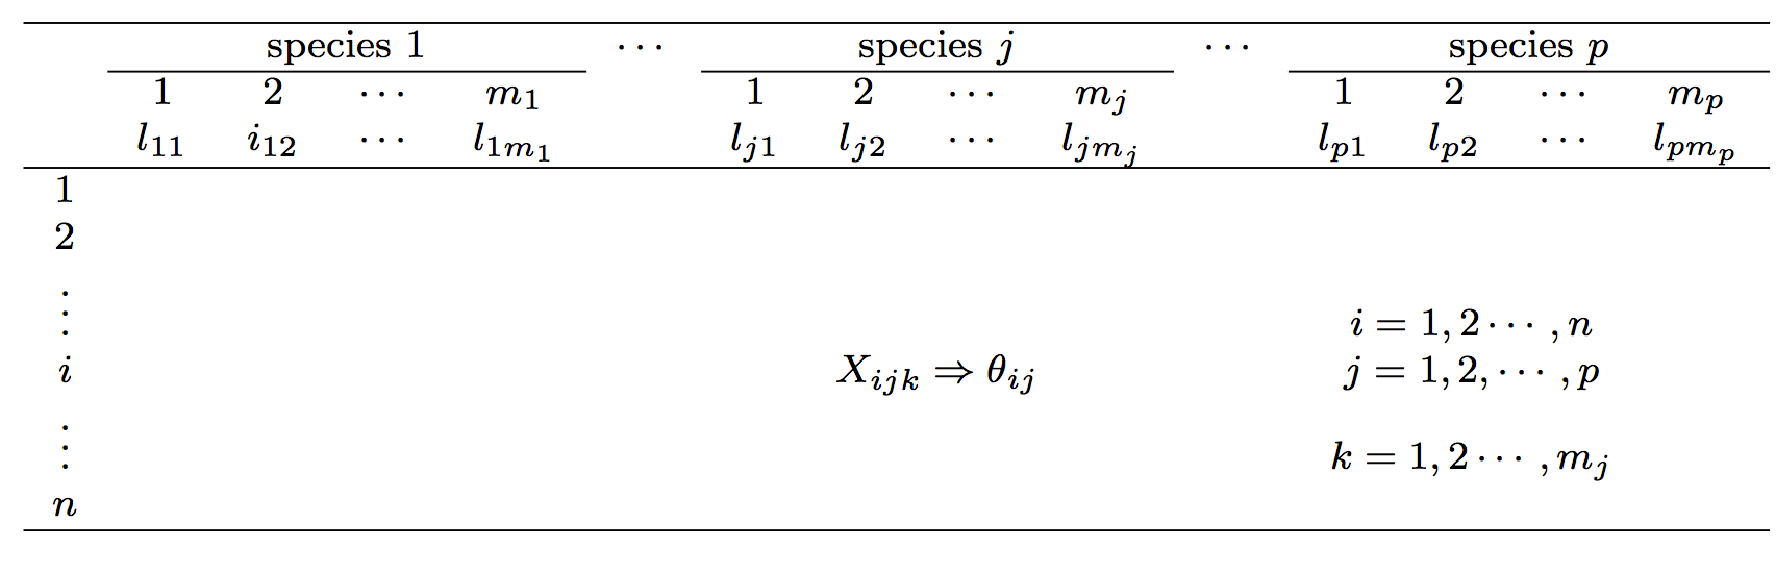
\includegraphics[scale=0.5,trim=0 0 0 0,clip]{Figure/F32_table.pdf}}
\caption[Summary of read count data that aligned to clade-specific markers]{Summary of read count data that aligned to clade-specific markers. The sequencing reads from $n$ metagenomic samples are aligned to a set of $m_j$ clade-specific marker genes for the $i$th species  for a total of $p$ species, where $X_{ijk}$ is  the number of reads that are assigned to the $k$th marker gene of the $j$th species for the $i$th sample.  $\theta_{ij}$ is the relative abundance of $j$th species in the $i$th sample and this is the parameter we want to estimate.}
\label{F32_table}
\end{figure*}


\begin{figure*}[htb]
	\centering
	%\adjustbox{trim={.15\width} {.06\height} {0.1\width} {.06\height},clip}%
	{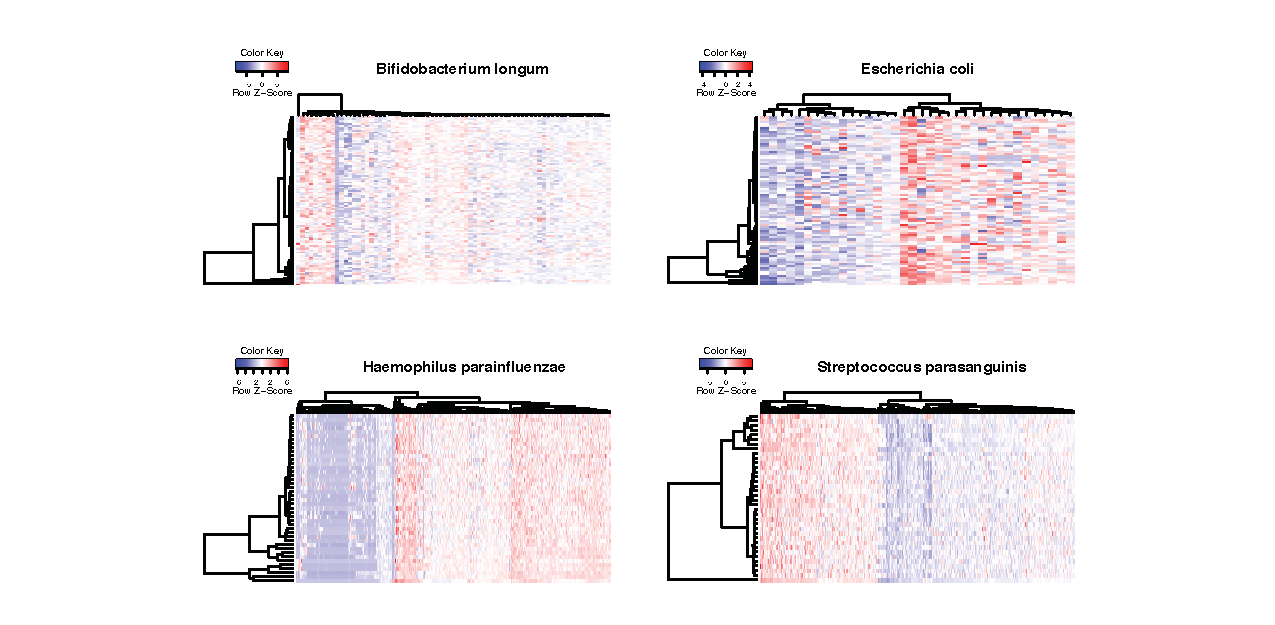
\includegraphics[scale=0.95,trim=80 0 0 0,clip]{Figure/F31_Marker_Effects.pdf}}
	\caption[Marker effects in the shotgun metagenomic data for four bacterial species]{Marker effects in the shotgun metagenomic data for four bacterial species. The raw sequencing reads were first aligned to the taxonomic markers and then normalized as the number of aligned read for each marker divided by marker length and total number of aligned reads for each sample. The normalized data was then clustered and showed in heatmap. The rows are  samples and columns are taxonomic markers from {\it MetaPhlAn}. }
	\label{F31_Marker_Effects}
\end{figure*}



\subsection{A multi-aample Poisson model to account for marker-specific effects}


Consider a metagenomic study with $N$ samples. After the sequencing reads are aligned to sets of clade-specific marker genes, the data can be summarized as a large table of counts as shown in Figure~\ref{F32_table}, where $X_{ijk}$ is  the count data of sequencing reads  for sample $i~(i = 1,2,\ldots,n)$, species $j~(j = 1,2,\ldots,p)$ and marker $k~(k = 1,2,\ldots,m_j)$. 
We model the count data for all species and all samples together and assume that the count  $X_{ijk}$ is generated from the following Poisson model,
\begin{equation*}
X_{ijk} \sim \mbox{Poisson}(\theta_{ij}t_{i}\phi_{jk}l_{jk}),
\end{equation*}
where $\theta_{ij} > 0$ is the relative abundance for the $j$th species in the $i$th sample. In common practice, the bacterial abundance are usually transformed into relative abundances (i.e. the bacterial abundance sum to 100\% in one sample).  We therefore impose that  $\sum_{j=1}^{p} \theta_{ij} = 1$. This constraint also avoids the identifiability issue in the model.  Here $t_i$ is the total read counts for sample $i$ that are mapped to the marker genes and $l_{jk}$ is the  length of the $k$th marker gene for $j$th species. Note that the species may have different number of markers. $t_i$ and $l_{jk}$ are known or can be calculated from the data directly.  The parameters $\phi_{jk} >0 ~(j=1, \cdots, p \textrm{ and } k=1,\cdots, m_j)$ are used to model  the market-specific effects for the set of  marker genes. The marker-specific effect can  be due to different GC contents, mappability and possible lateral gene transfers.  Our model uses data from multiple samples to estimate the marker effects $\phi_{jk}$.  When $\phi_{jk}=1$, our model is a Poisson model without considering the marker effects, which is essentially the approach used by {\it MetaPhlAn}.


\subsection{Model fitting}
We fit the model  and estimate the parameter using the maximum likelihood estimation, where the   likelihood   function is
\begin{align*}
L & = \prod_i\prod_j\prod_k \frac{e^{-\theta_{ij}t_{i}\phi_{jk}l_{jk}}(\theta_{ij}t_{i}\phi_{jk}l_{jk})^{x_{ijk}}}{x_{ijk}!},
\end{align*}
and its logarithm is 
\begin{align*}
\log L =  &  
\sum_i\sum_j\sum_k (-\theta_{ij}t_{i}\phi_{jk}l_{jk}+x_{ijk}log(\theta_{ij}t_{i}\phi_{jk}l_{jk})-log(x_{ijk}!)).
\end{align*}
Estimates $\theta$ and $\phi$ can be obtained iteratively.  We  first estimate all $\theta_{ij}$ by fixing  $\phi_{ik}$ at the current values, 
\begin{align*}
\hat \theta_{ij} = \frac{\sum_kx_{ijk}}{t_{i}\sum_k\phi_{jk}l_{jk}}, 
\end{align*}
and then normalize these values so that $\sum_{j=1}^p\hat{\theta}_{ij}=1$ for $i=1,\cdots, n$.
We estimate all $\phi_{ik}$ by fixing  $\theta_{ij}$ at the current values, 
\begin{align*}
\hat \phi_{ik} = \frac{\sum_ix_{ijk}}{l_{jk}\sum_i\theta_{ij}t_{i}}.
\end{align*}

We iteratively update  $\theta_{ij}$ and $\phi_{ik}$ until convergence. Since the closed-form updating formula are available, the algorithm is very efficient. 




\section{Simulation studies}
%\subsection{Simulation based on the multi-sample Poisson model}
We  first performed  a simulation study to examine the model fitting, where we simulated different sample size $n=(20,50,100)$ and different number of markers $m=(20,50,100)$ per species. In order to mimic the skewed distribution of species abundance in a sample, we simulated $\theta_{ij}$ from a log-normal distribution with $\mu=0$ and $sd=1.5$. The simulated $\theta_{ij}$ were then normalized so that    $\sum_{j=1}^{p} \theta_{ij} = 1$. The scaled marker length $l_{jk}$ and total read counts $t_i$ was simulated uniformly from [0.1,10] and [50,500], respectively. We simulated $\phi_{jk}$ from a log-normal distribution with $\mu=0$ and $sd= 1.5$. We fitted the MSSQ model on the simulated data and  then calculate the average relative difference (AVGRD) for  $\hat\theta$ and $\hat\phi$, which is defined as
$$\frac{1}{n}\sum_i^n \frac{|\theta_{ij}-\hat{\theta}_{ij}|}{\hat{\theta}_{ij}}, \mbox{  }
\frac{1}{m}\sum_k^m \frac{|\phi_{jk}-\hat{\phi}_{jk}|}{\hat{\phi}_{jk}}.
$$ 
The simulations were repeated 1,000 times for each combination of sample size and marker size. The mean and standard error of the AVGRD over 1000 repeated simulations were then calculated and reported.

Table~\ref{MSSQTable1} shows the simulation results. When the number of markers per species is fixed, increasing  sample size improves the estimation accuracy of both $\theta$ and $\phi$. Similarly, when the sample size is fixed, more markers can improve the estimation accuracy of both $\theta$ and $\phi$.

\begin{table}[ht]
	\caption[Parameter estimation for data simulated from the multi-sample Poisson model]{Parameter estimation for data simulated from the multi-sample Poisson model with different sample size $n$ and different marker size $m$.  For each parameter, the mean and standard error (SE) of average relative difference (AVGRD) are calculated based on 1000 replications. For each $n$ and $m$, the first row are estimates for $\theta$; the second row are for $\phi$.   
		\label{MSSQTable1}}
	\begin{center}	\begin{tabular}{lrrrrrrrrrr}
			\hline
			AVGRD& & \multicolumn{2}{c}{$m = 20$} & \multicolumn{2}{c}{$m = 50$}  & \multicolumn{2}{c}{$m = 100$}    \\
			\cline{3-8}
			& & mean & SE & mean & SE & mean &  SE &  \\
			%%%%
			%%%%
			\hline
			%%%%
			$n$=20 & $\theta$ & 0.19 & 0.05 & 0.14 & 0.04 & 0.11 & 0.03  \\
			& $\phi$ & 0.22 & 0.07 & 0.16 & 0.05 & 0.13 & 0.03  \\
			$n$=50 & $\theta$ & 0.09 & 0.02 & 0.07 & 0.01 & 0.06 & 0.01  \\
			& $\phi$ & 0.08 & 0.02 & 0.07 & 0.02 & 0.07 & 0.01  \\
			$n$=100 & $\theta$ & 0.06 & 0.01 & 0.05 & 0.01 & 0.04 & 0.01  \\
			& $\phi$ & 0.04 & 0.01 & 0.04 & 0.01 & 0.04 & 0.01  \\
			
			%%%%%
			%%%%%
			\hline
		\end{tabular}
	\end{center}
\end{table}


We next  studied the effects of allowing the marker-specific effects in the Poisson on species abundance quantification, where we simulated $n=50$ samples and each sample had $p=50$ species.  The true abundance $\theta_{ij}$, the scaled marker length $l_{jk}$ and total read counts $t_i$ were simulated in the  same way  as previously. For each species, the number of markers $m_j$ was uniformly simulated from [10,50]. To mimic  different degrees of marker effects, we simulated $\phi_{jk}$ from a log-normal distribution with $\mu=0$ and $sd=(0, 0.5, 1, 1.5)$ for four different simulation settings, respectively. The simulation setting with log-normal($\mu=0$, $sd=0$) indicates no marker effect in the data and the other three settings indicate increasing marker effects.


We observed that ignoring the marker-specific effects led to large biases in  the estimates of the abundance $\theta_{ij}$, as shown in Figure \ref{F33_2016_02_07_Abundance_Estimation_Scale5_100_Merge} (full-scale in upper panel and zoomed-in to 0-5\% scale in lower panel). When the marker effect increases, the estimated abundance deviated more from the true abundance, where the mean of AVGRD were  0.07, 0.15, 0.28, 0.52.  In contrast, estimates of the relative abundances from MSSQ showed  little biases when there were strong maker-specific effects. The mean of AVGRD were 0.07, 0.09, 0.09, 0.10, respectively. 

\begin{figure*}[ht]
	\centering
	%\adjustbox{trim={.0\width} {.15\height} {.0\width} {.0\height},clip}%
	{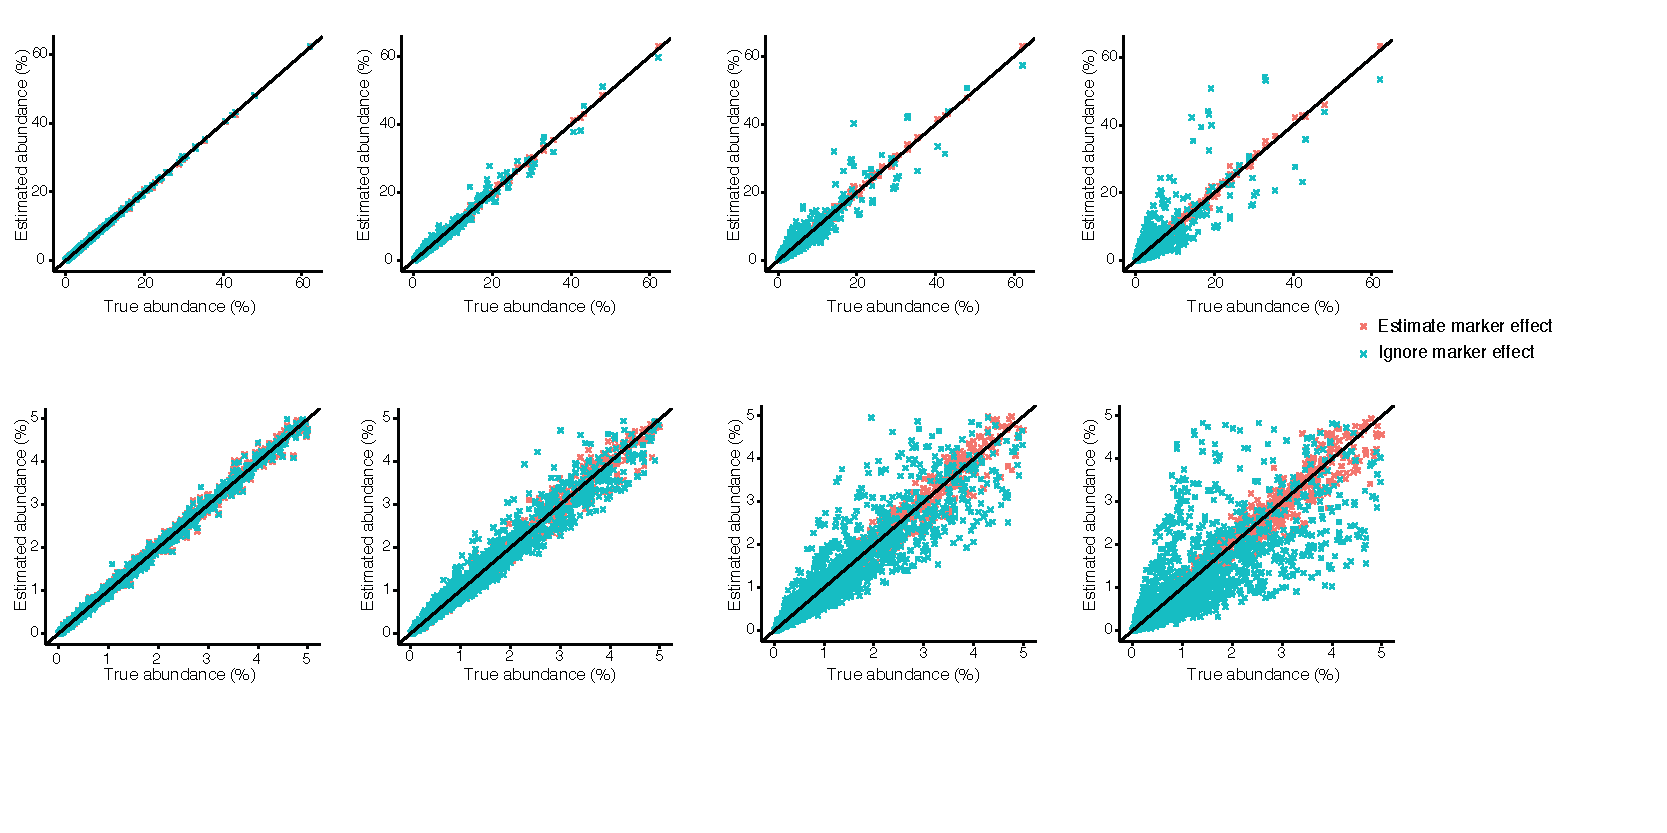
\includegraphics[scale=0.53,trim=0 60 20 0,clip]{Figure/F33_2016_02_07_Abundance_Estimation_Scale5_100_Merge.pdf}}
	\caption[Comparison of relative abundance estimation by MSSQ  with and without estimating marker effect]{Comparison of relative abundance estimation by MSSQ  with and without estimating marker effect ($\phi_{jk}=1$) for four scenarios with increasing marker-specific effects (from left to right). A total of 50 samples, each with 50 species were simulated. Upper panel, full scale; lower panel, zoom-in 0-5\% scale  }
	\label{F33_2016_02_07_Abundance_Estimation_Scale5_100_Merge}
\end{figure*}



\section{Application to the human gut microbiome data}
\label{sec:realdata}
\subsection{Data description and processing} 
We applied MSSQ to a data set of shotgun metagenomic study comparing gut microbiome between healthy children and children with Crohn's disease \citep{lewis2015inflammation,lee2015comparative}. A total of 90 children with  Crohn's disease  and 26 healthy controls were recruited to the study and  provided fecal samples for  shotgun metagenomic sequencing.  DNAs were prepared from whole stool and were sequenced using the Illumina HiSeq paired-end method, resulting in an average number of reads per sample of $11 \times 10^6$ with an average length 100 bases on each end of the paired-end read. We were  interested in quantifying the bacterial abundances and identifying the  bacteria species that show differential abundance between the normal samples and the Crohn's disease samples.


We first aligned the sequencing reads  to the {\it MetaPhlAn} clade specific markers for each of the bacterial species.  In order to compare our method with {\it MetaPhlAn}, we applied the same filtering criteria used by {\it MetaPhlAn}. Specifically,  for each species, we filtered out the upper 10\% percentile of the most abundant markers and lower 10\% percentile least abundant markers. We replaced the read counts of those filtered markers with NAs and our model ignores the NAs in the model fitting procedure. We ran  {\it MetaPhlAn} on the same data set and compare the results with those from MSSQ.


\subsection{Abundance estimation with MSSQ}
After the filtering steps, we applied MSSQ to  quantify the  species abundance from healthy children and those with Crohn's disease separately. MSSQ identified a total of 138 species presented in the control samples and 216 in the disease samples.  {\it MetaPhlAn} identified the same number of species in control and disease samples. 


We then compared the abundance estimation by MSSQ and {\it MetaPhlAn} (Figure~\ref{PLEASE_COMBO_Abundance_Estimation}). When  the marker-specific  effects were excluded from the model, i.e., setting all $\phi_{jk}$=1, as expected, MSSQ resulted in  the same abundance estimate as the {\it MetaPhlAn} for both control and disease samples. When the marker-specific  effects were estimated, MSSQ shows different abundance estimation from  {\it MetaPhlAn}. Overall, we observed that the estimates from both methods were comparable with a Pearson correlation of 0.92 (See Figure \ref{PLEASE_COMBO_Abundance_Estimation} upper panel). However, for low abundant species, a large discrepancies of the estimates were observed (Figure \ref{PLEASE_COMBO_Abundance_Estimation} lower panel).  Due to low read counts to these species, a large variability in these estimates were expected. The overall pattern was similar to our simulation results in Figure \ref{F33_2016_02_07_Abundance_Estimation_Scale5_100_Merge}. We also observed that the differences were greater in disease samples than in the control samples.

\begin{figure}[ht]
\centering
{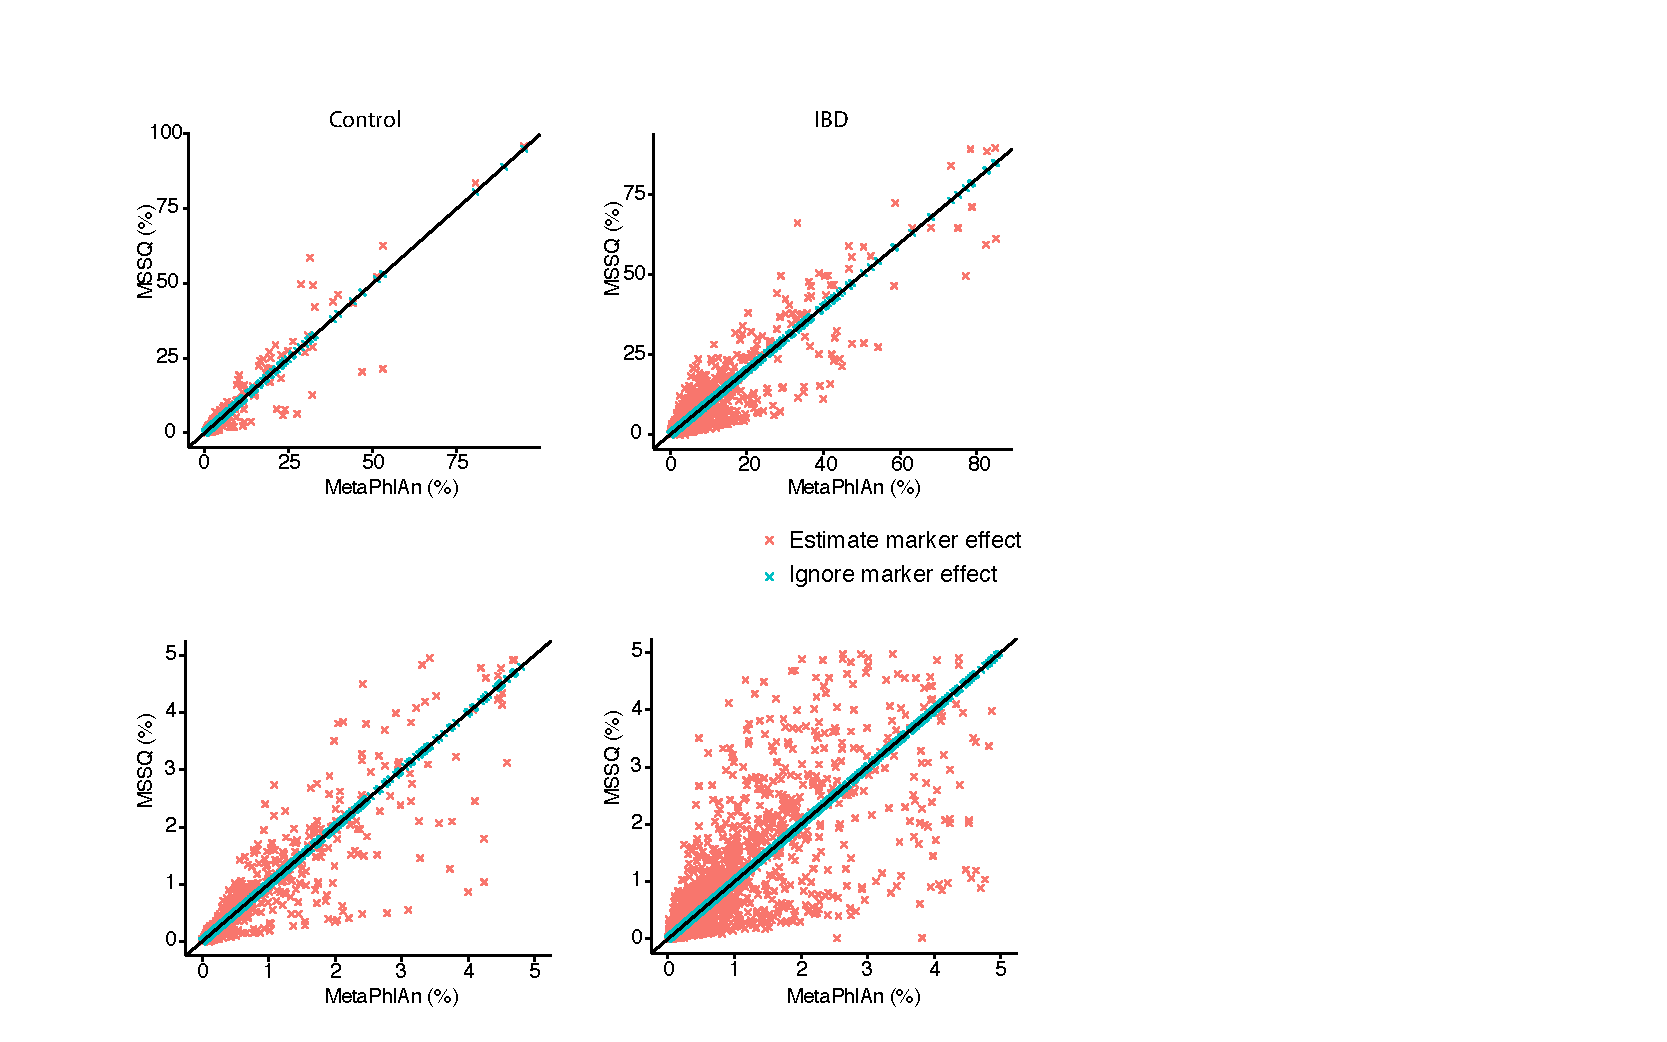
\includegraphics[scale=0.8,trim=20 10 150 0,clip]
{Figure/F34_2016_02_01_PLEASE_COMBO_Abundance_Estimation_Merge.pdf}
}
\caption[Comparison of estimated relative abundances from MSSQ and {\it MetaPhlAn}]{Comparison of estimated relative abundances from MSSQ and {\it MetaPhlAn}. Upper panel: all species; Lower panel: species with abundances $<5\%$. }
\label{PLEASE_COMBO_Abundance_Estimation}
\end{figure}


\subsection{Clustering and differential abundance analysis}
We next evaluated whether the abundance quantification by MSSQ can improve the downstream analysis such as clustering and differential abundance analysis. Before we performed the downstream analysis, we first filtered out the rare species, which is a common pre-processing procedure  often used in the literature \citep{Kostic:2015bh,Romero:2014il,Stein:2013dl}. Particularly, the species with an estimated abundance $< 1\%$ in all the control and disease samples in both MSSQ and {\it MetaPhlAn} estimation were filtered out. After filtering, 136 species were left for following analysis. 

Figure \ref{F35_2016_02_01_Heatmap_Merge} shows the heatmap of the estimated abundances from MSSQ and {\it MetaPhlAn}, where the samples were clustered with  Bray-Curtis distance and the species were clustered based on Pearson's correlations. We observed a clear separation of normal and Crohn's disease gut microbiome samples based on {\it MetaPhlAn} and MSSQ estimation of the species abundances.  However, the clustering results based on the MSSQ estimation show a clearer pattern. 




\begin{figure*}[th]
	\centering
	{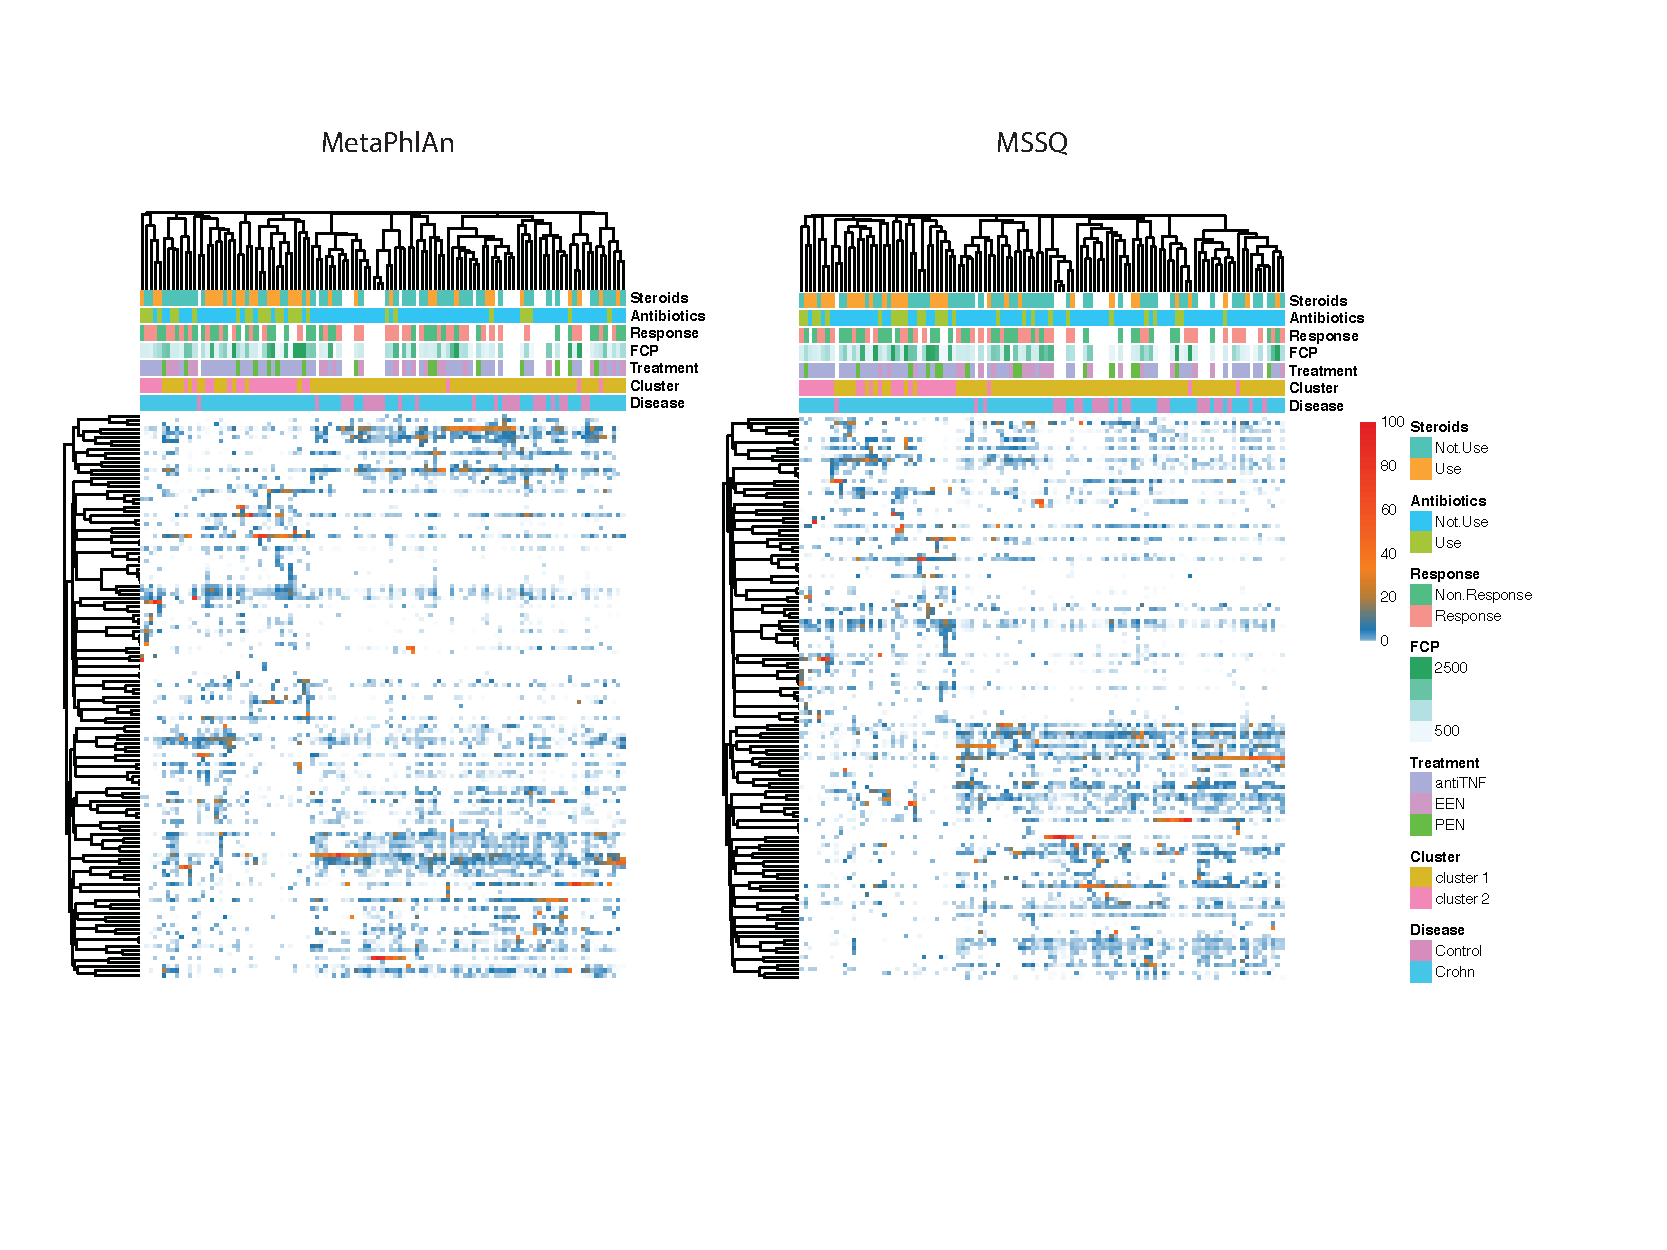
\includegraphics[scale=0.6,trim=30 140 0 0,clip]{Figure/F35_2016_02_01_Heatmap_Merge.pdf}
	}
	\caption[Heatmap of the estimated abundances from MSSQ and {\it MetaPhlAn}]{Heatmap of the estimated abundances from MSSQ and {\it MetaPhlAn} based on analysis of metagenomic data comparing normal samples and those with Crohn's disease.  Clinical meta-data are presented in the top bars. See \cite{lewis2015inflammation} and \cite{lee2015comparative} for details of the clinical meta-data. }
	\label{F35_2016_02_01_Heatmap_Merge}
\end{figure*}


As a comparison, we also tested for differential abundance between control and disease samples for each species using the Wilcoxon rank-sum test. Using these estimated abundance from {\it MetaPhlAn}, Wilcoxon rank-sum test identified 39 differentially abundant species with  FDR adjusted $p$-value $<$ 0.05. Based on the estimated abundance from MSSQ, 41 species were identified to be differentially abundant between control and disease samples, including all 39 differentially abundant species identified based on the {\it MetaPhlAn} estimation. Among the species that are more abundant in Crohn's patients, {\it E. coli, Bacteroides, Enterococcus, Klebsiella}, and {\it  Ruminococcus gnavus} have been reported in literature \citep{Sartor, Liu95}. Among the protective species, {\it Bifidobacterium, Roseburia} and {\it Eubacterium} were also reported in previous studies \citep{manichanh2012gut}. \cite{manichanh2012gut} detected {\it Lactobacillus} as a protective species that was more abundant in normal gut. 

The two species that were only identified when MSSQ was applied include  {\it Coprococcus comes}, which belongs to genera {\it Coprococcus}, and {\it Clostridium symbiosum}. Both  species were reported to be associated with dysbiosis, CD \citep{gevers2014treatment} and UC \citep{du2015development}.  {\it Clostridium symbiosum} has been reported to protect the gut mucosa by producing butyrate \citep{van2013butyrate}.


\subsection{Comparing marker effect in control and disease samples}
Figure~\ref{F33_Marker_Effect_Boxplot} shows the estimated marker effect $\hat{\phi}$ for each species in normal control and disease samples. The dispersion of $\hat{\phi}$ values indicates the marker effects indeed present in the real data. The average dispersion of $\hat{\phi}$ is 43.10 for species in control samples and 729.12 for species in disease samples, where the dispersion was measured by the standard deviation. 

\citet{Korem:2015cv} studied the bacterial growth dynamics using shotgun metagenomic data. They observed that when the bacteria is in replication status, the read coverage is not uniformly distributed across the bacterial genome. They further showed that bacterial growth dynamics are associated with diseases such as diabetes and Crohn's disease. Specifically, they found that the growth dynamics of two bacterial species Bifidobacterium longum and Escherichia coli are associated with Crohn's disease. We are interested to see if our model can capture the bacterial growth dynamics. We examined the estimated marker effects ($\phi$) for those two species between control and Crohn's disease samples in our metagenomic study (Figure~\ref{F36_Science_Five_Species}). We also plotted the estimated marker effects from several non-association species in \citet{Korem:2015cv} as negative control. Interestingly, the marker effects estimated from MSSQ show great difference between control and disease groups. No significant difference is observed for the other negative controls. This result indicate that marker effects ($\phi$) from MSSQ capture the bacterial growth dynamics and the difference in growth rate is associated with disease status. The bacterial relative abundance and growth dynamics are not necessarily correlated. MSSQ captures these two biological features.

\begin{figure*}[p]
	\centering
	{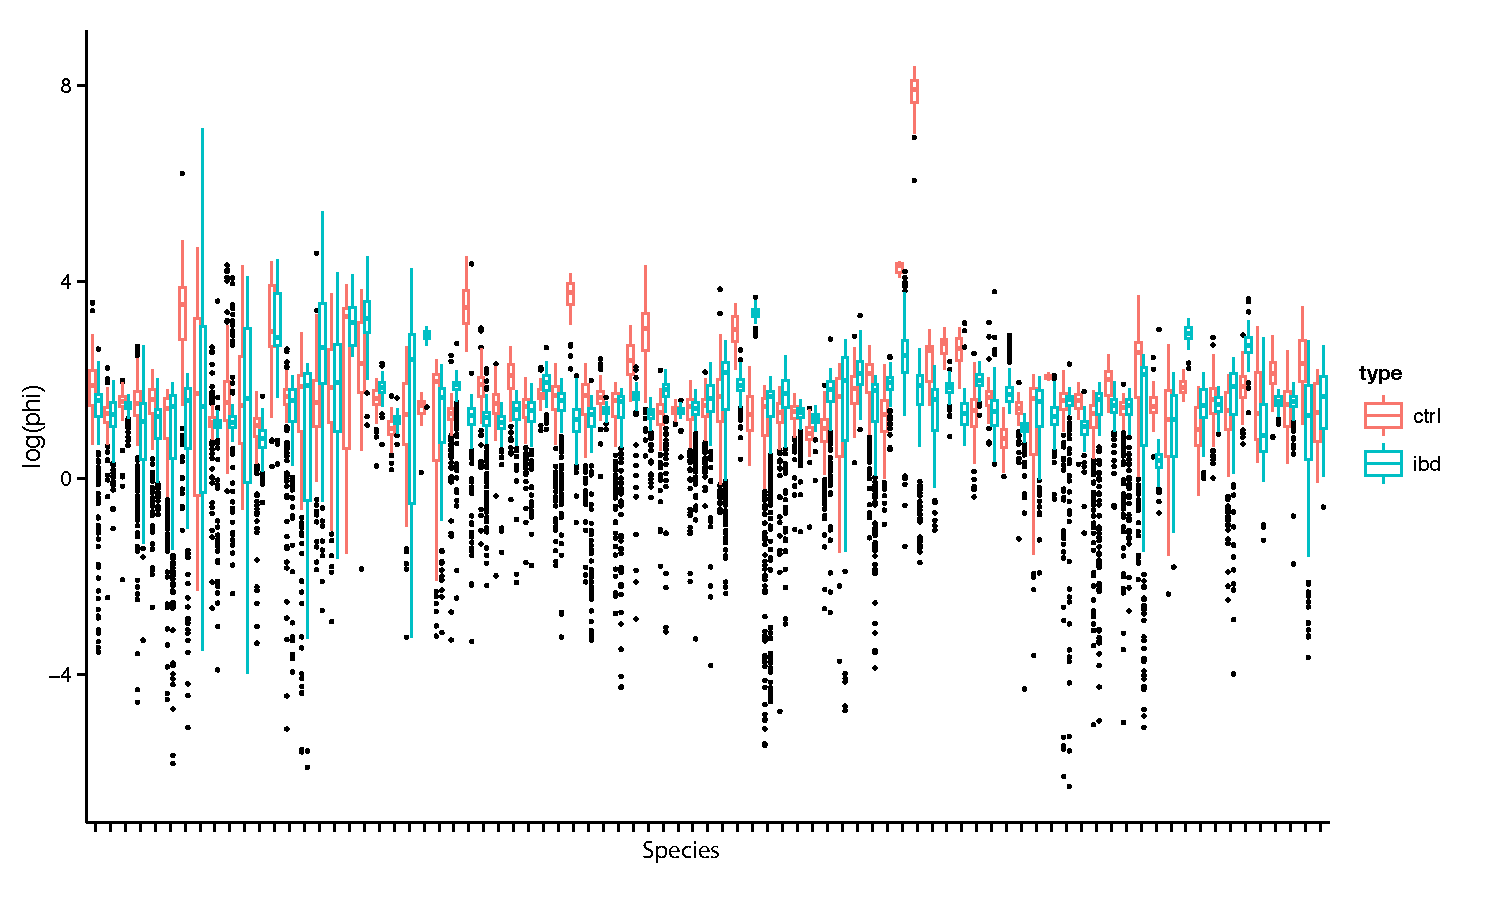
\includegraphics[scale=0.6,trim=0 20 0 0,clip]{Figure/F33_Marker_Effect_Boxplot.pdf}
	}
	\caption[Distribution of estimated marker-specific effects]{Distribution of estimated marker-specific effects for each species in the control samples  (upper panel) and disease samples (lower panel). Each dot represents the estimated $\phi$ with log transformation and each boxplot represents a species.}
	\label{F33_Marker_Effect_Boxplot}
\end{figure*}


\begin{figure*}[p]
	\centering
	%\adjustbox{trim={.0\width} {.0\height} {0.0\width} {.0\height},clip}%
	{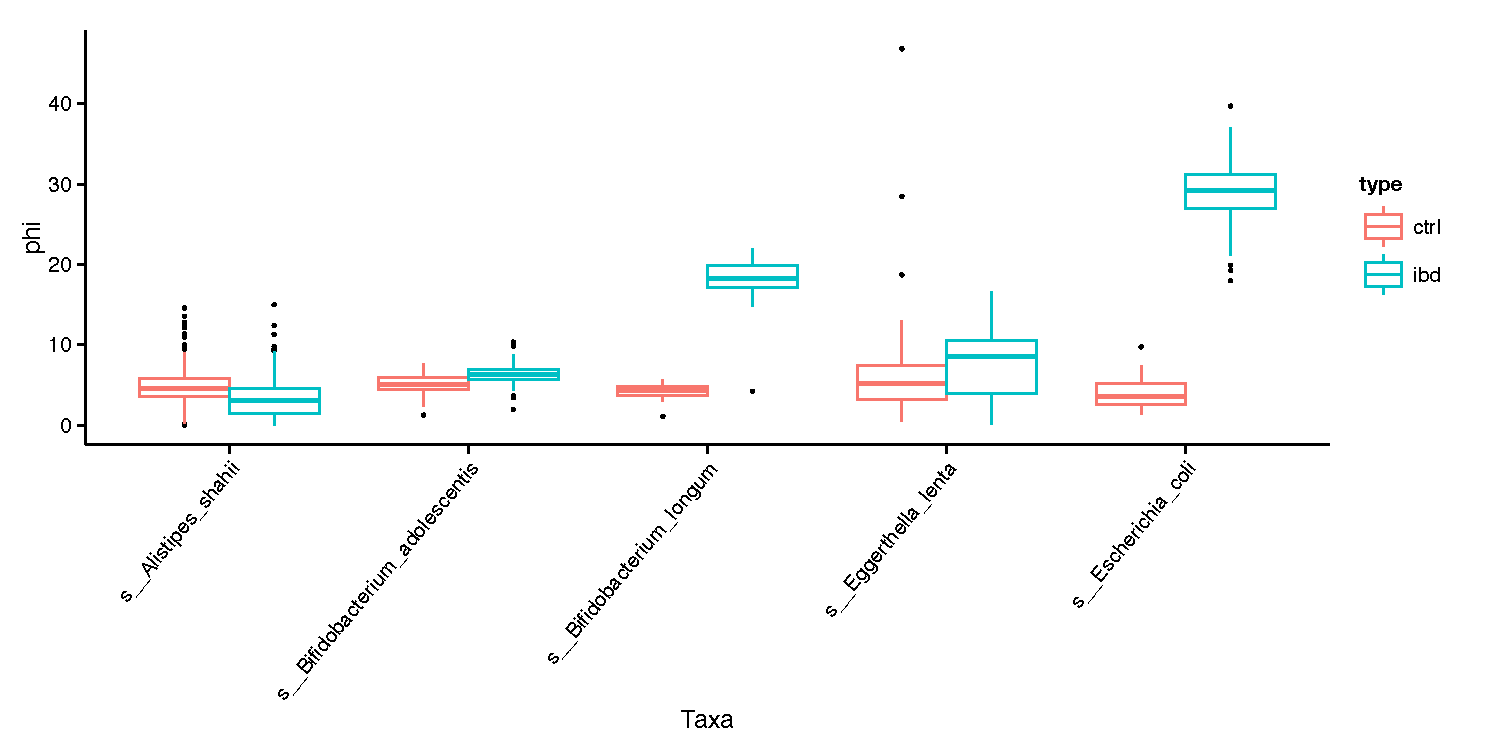
\includegraphics[scale=0.55]{Figure/F36_Science_Five_Species.pdf}
	}
	\caption[MSSQ captures the bacterial growth dynamics]{MSSQ capture the bacterial growth dynamics. \citet{Korem:2015cv} showed the growth dynamics of two bacterial species Bifidobacterium longum and Escherichia coli are associated with Crohn's disease. The estimated marker effects ($\phi$) for those two species between control and Crohn's disease samples in our metagenomic study are plotted. Three non-association species in \citet{Korem:2015cv} are also plotted as negative control.}
	\label{F36_Science_Five_Species}
\end{figure*}




\section{Discussion}
We have proposed a multi-sample Poisson model to quantify the bacterial abundances based on the shotgun metagenomic data.  Our method uses the count data of reads  aligned to clad-specific  marker genes  to quantify  the species abundances,  taking into account the marker effects that are observed in the shotgun sequencing data. In our analysis of real data, we used the marker genes sets used in  {\it MetaPhlAn} package.  Alternatively, one can also use the 40 universal marker genes defined by \cite{Sunagawa:2013if}. It would be interesting to compare whether different marker genes lead to similar species quantification. 
Simulation results indicate that the proposed model-based approach can lead to better quantification of species abundances.

We further demonstrated the proposed methods in an analysis of pediatric gut microbiome to identify the species that are associated with Crohn's disease. The discrepancy of the differential abundant species identified by MSSQ and {\it MetaPhlAn} is due to whether the maker-specific effects are accounted in the estimation. Our simulations have clearly demonstrated the ignoring such marker-specific effects can lead to biased quantification of the species abundances. The marker-specific effects could originates  from different sources. For example, it is well known that the sequencing reads are not uniformly distributed among genomic regions and are correlated with GC contents of the genomic regions \citep{ross2013characterizing}. Further, the copy number variation of the genes can also contribute to the under- or over- presentation of certain gene regions. Sequencing error and alignment error are other potential sources for non-uniform distribution of the reads and may cause the large  marker-to-marker variability we observed in the data. 

In our analysis, we fitted the multi-sample Poisson model for all the species and all the samples simultaneously. Since we do not expect to observe all the species in all the samples,  some regularization on the relative abundance parameter $\theta_{ij}$ may help to improve  the abundance quantification. Finally, it is interesting to establish the asymptotic distribution of the resulting estimates of the relative abundances when both the sample size $n$ and the numbers of marker genes $m_j$ go to infinity. 
